\subsection{Use Case Formulation}

Before the use cases executed in Table \ref{tbl:use_cases} were developed, there were thousands of transactions executed with a variety of parameters. These initial use cases helped us develop the ideal use cases that would best show the benefits and drawbacks of the new dynamic reputation solution.

For the graphs in this section we use the term \textbf{affected transactions} to identify transactions that were aborted prematurely in the system.

Table \ref{tbl:use_cases_initial} shows the use cases that were executed initially to get a baseline of how transactions within the system would be affected, when a recalculation would occur, and what was the impact of that recalculation.

\begin{table}
\captionsetup{justification=centering}
\centering
 \begin{tabular}{|| c | c | c | c | c ||} 
 \hline
 \textbf{Name} & \textbf{Total \#} & \textbf{Recalculation \%} &  \textbf{Conflict \%} & \textbf{Abort \%} \\ [0.5ex] 
 \hline\hline
 Use Case Alpha & $\approx$ 23,000 & 50 & 10 & 5  \\ 
 \hline
 Use Case Beta & $\approx$ 2,500 & 10 & 25 & 25  \\ 
 \hline
 Use Case Gamma & $\approx$ 1,900 & 5 & 40 & 40  \\ 
 \hline
 Use Case Delta & $\approx$ 1,200 & 7 & 50 & 50  \\ 
 [1ex] 
 \hline
\end{tabular}
\caption{Initial Use Cases}
\label{tbl:use_cases_initial} % label to refer figure in text
\end{table}

Our very first use case (Use Case Alpha shown in Figure \ref{image:use_case_alpha}) started with a high recalculation percentage to get a baseline test of the prototype. What we saw with such a high recalculation percentage was that the affected transactions spike to approximately 3\% and then began to level off as the number of transactions within the system increased. We then realized that with those parameters a recalculation would never be triggered and the system would continue on.

\begin{figure}
\centering
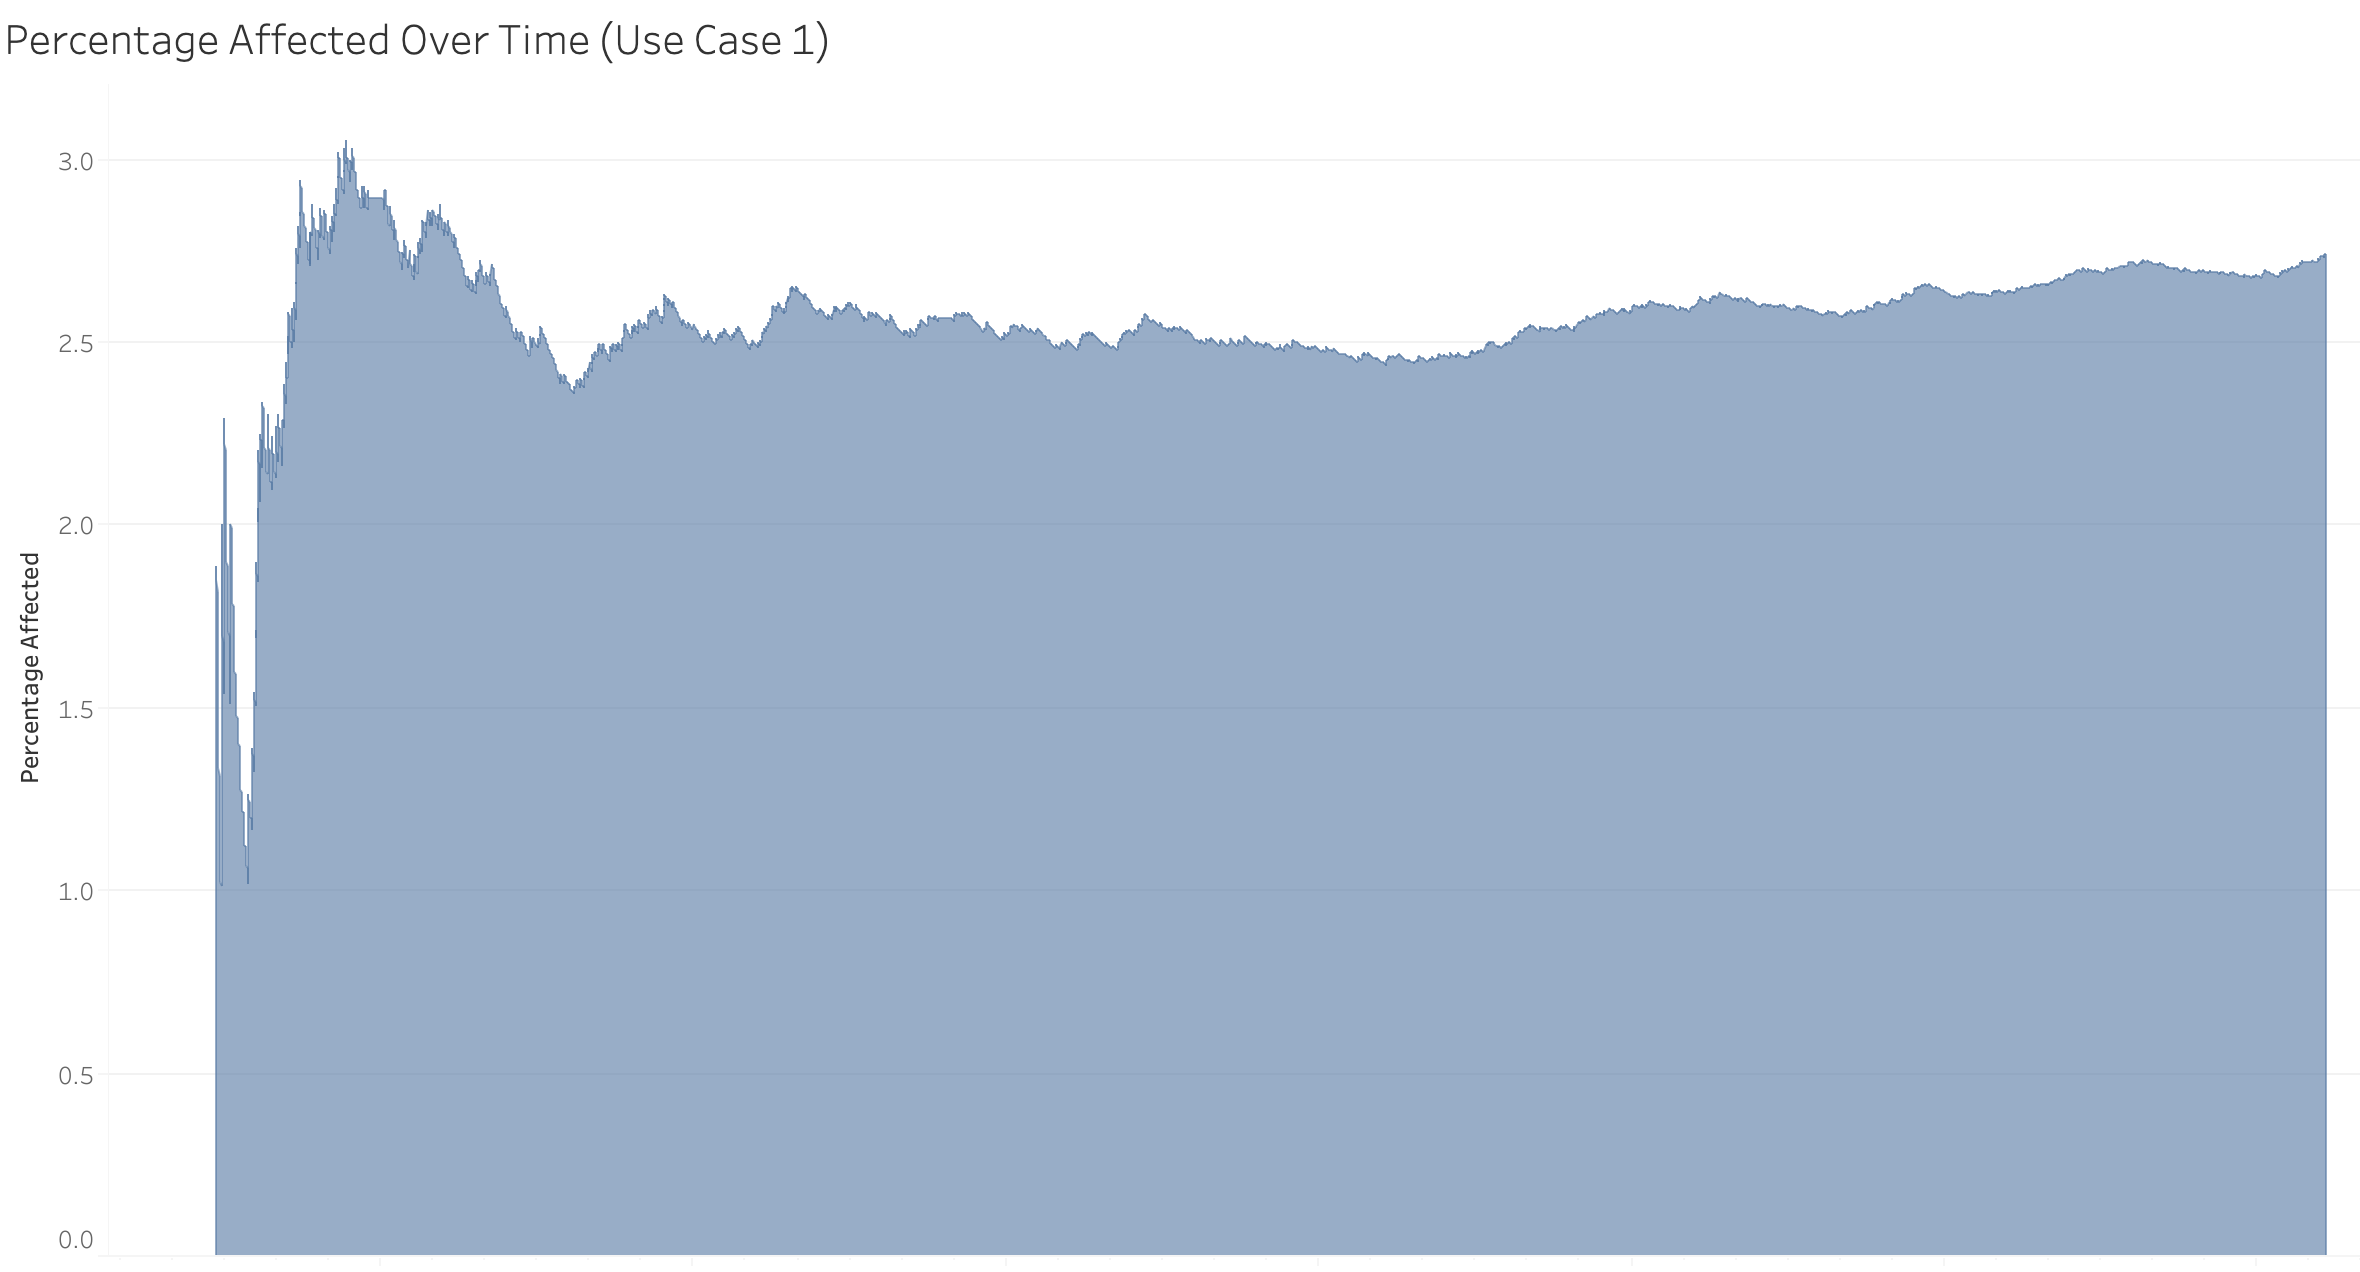
\includegraphics[scale=0.35]{images/UseCase1.png}
\caption{Use Case Alpha}
\label{image:use_case_alpha}
\end{figure}

Our next use case (Use Case Beta shown in Figure \ref{image:use_case_beta}) decreased the recalculation to 10\% while increasing the conflicting and abort percentages in the system to 25\%. This was enough of a change to cause a single recalculation in the beginning but as the number of transactions increased in the system the number of affected transactions would grow too slowly to initiate another recalculation.

\begin{figure}
\centering
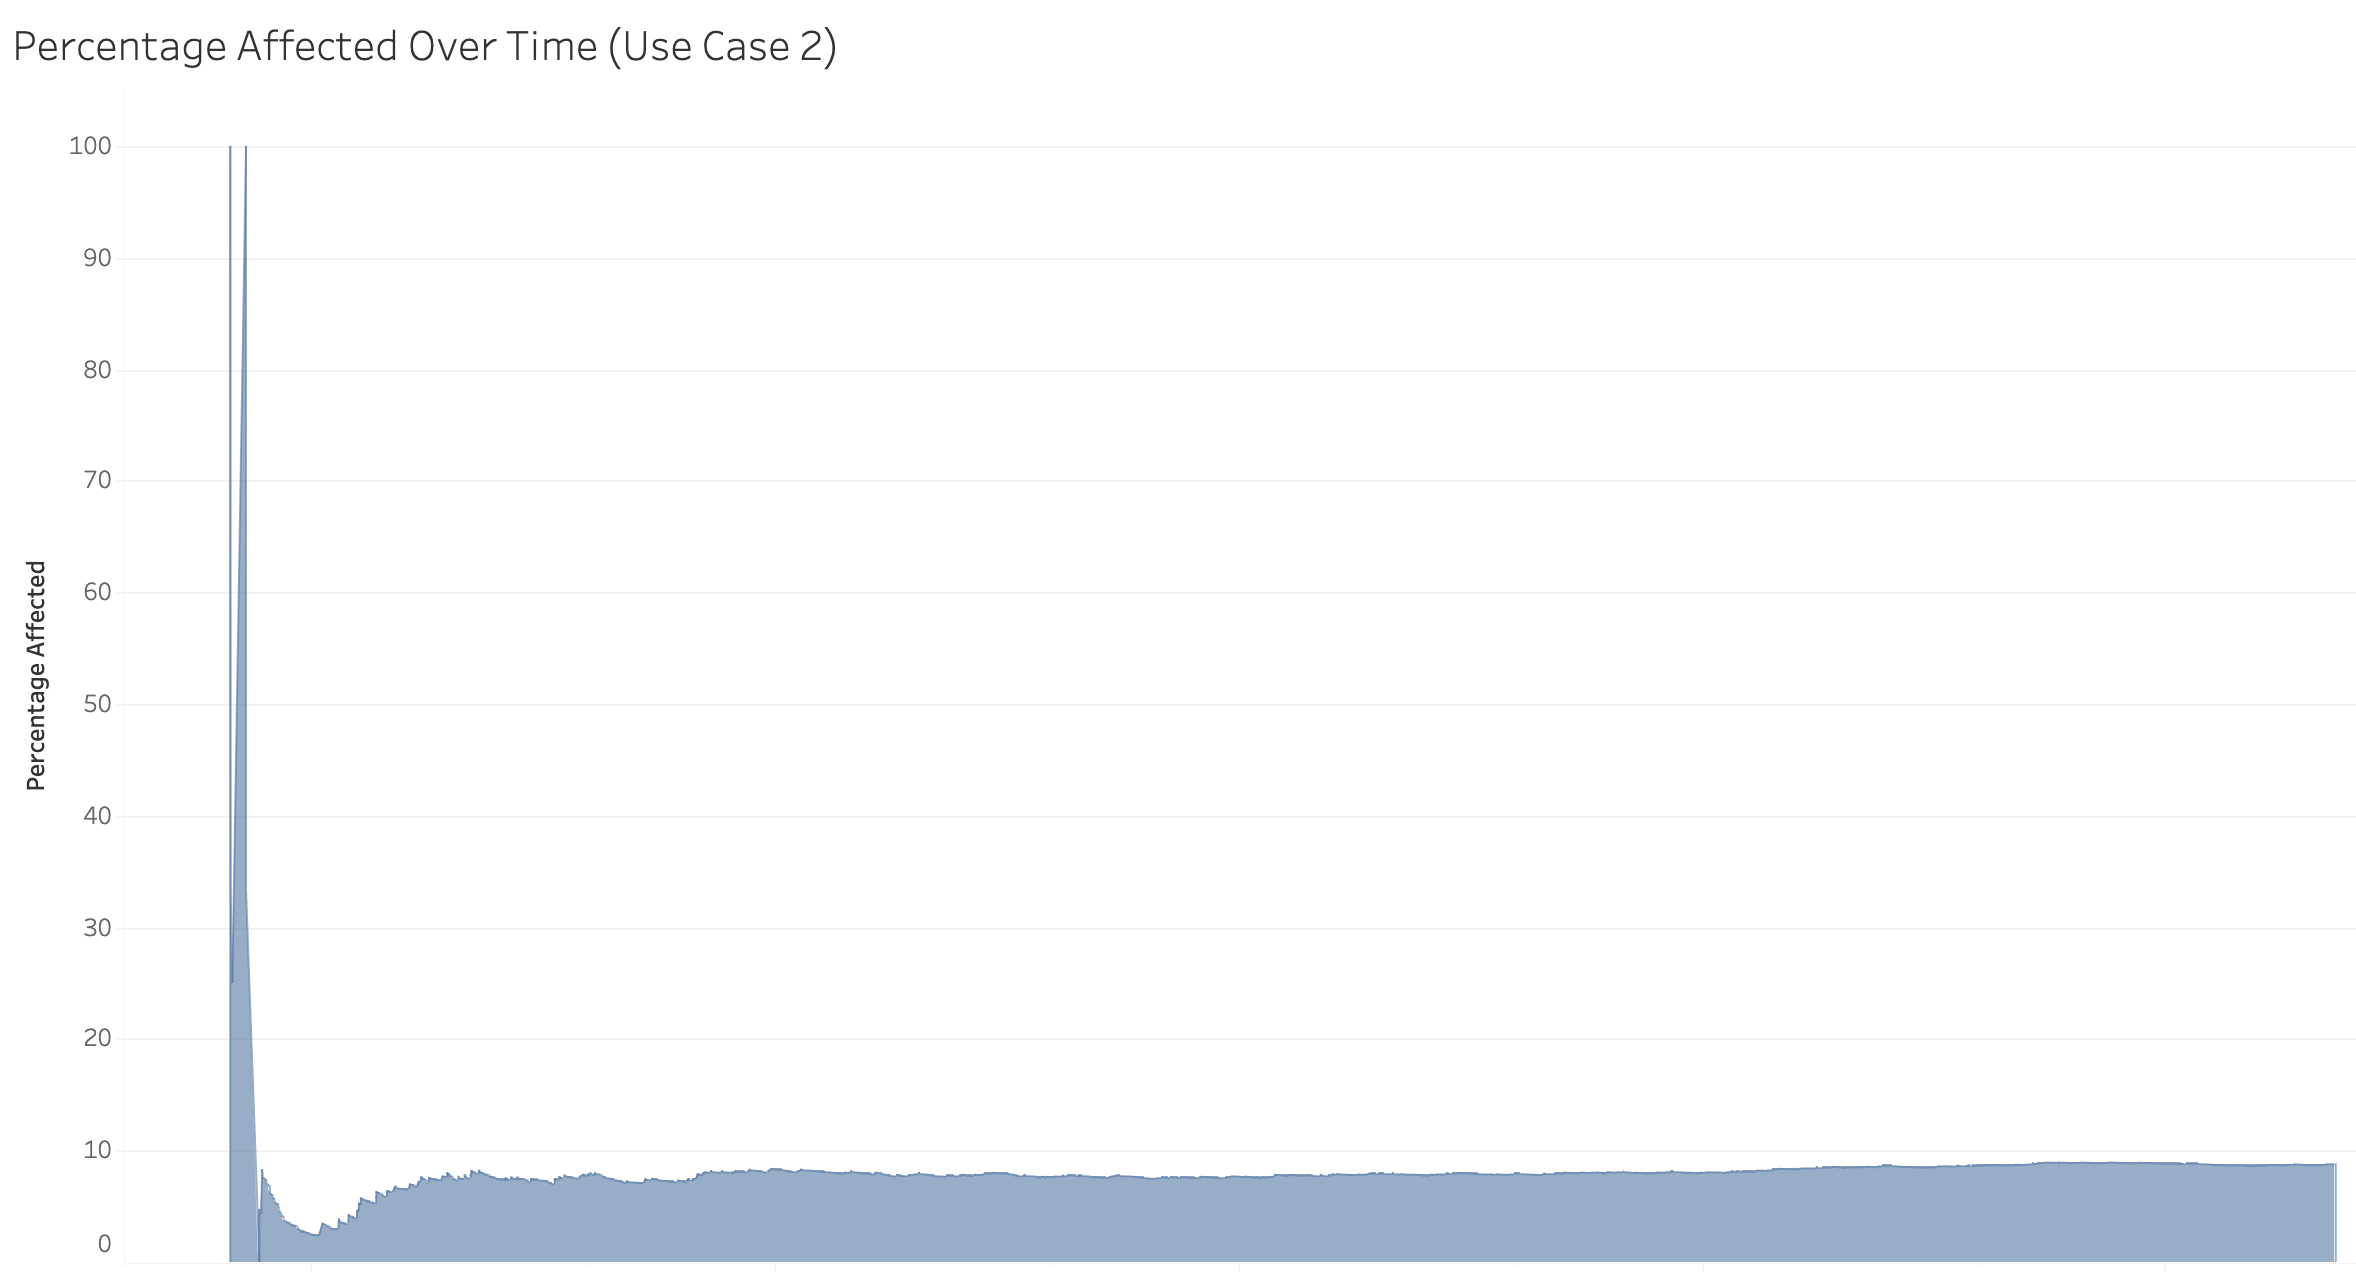
\includegraphics[scale=0.35]{images/UseCase2.png}
\caption{Use Case Beta}
\label{image:use_case_beta}
\end{figure}

After seeing the results from Use Case Beta we set the parameters of the next execution to be a bit more exaggerated. Use Case Gamma (shown in Figure \ref{image:use_case_gamma}) lowers the recalculation percentage to 5\% while the conflicting and abort percentages were set much higher at 40\%. What you can see from the graph is that the affected transactions spike to 100\% which kicks off a recalculation of the rankings within the system. After the recalculation the numbers are reset but the conflicting and abort percentages are so high that it continues spiking the affected transactions to 100\%. This repetition of spikes continues throughout the entire execution. While Use Case Gamma is not an ideal system that transactions will execute within, it gave us a upper bound of what happens when there is a large percentage of affected transactions.

\begin{figure}
\centering
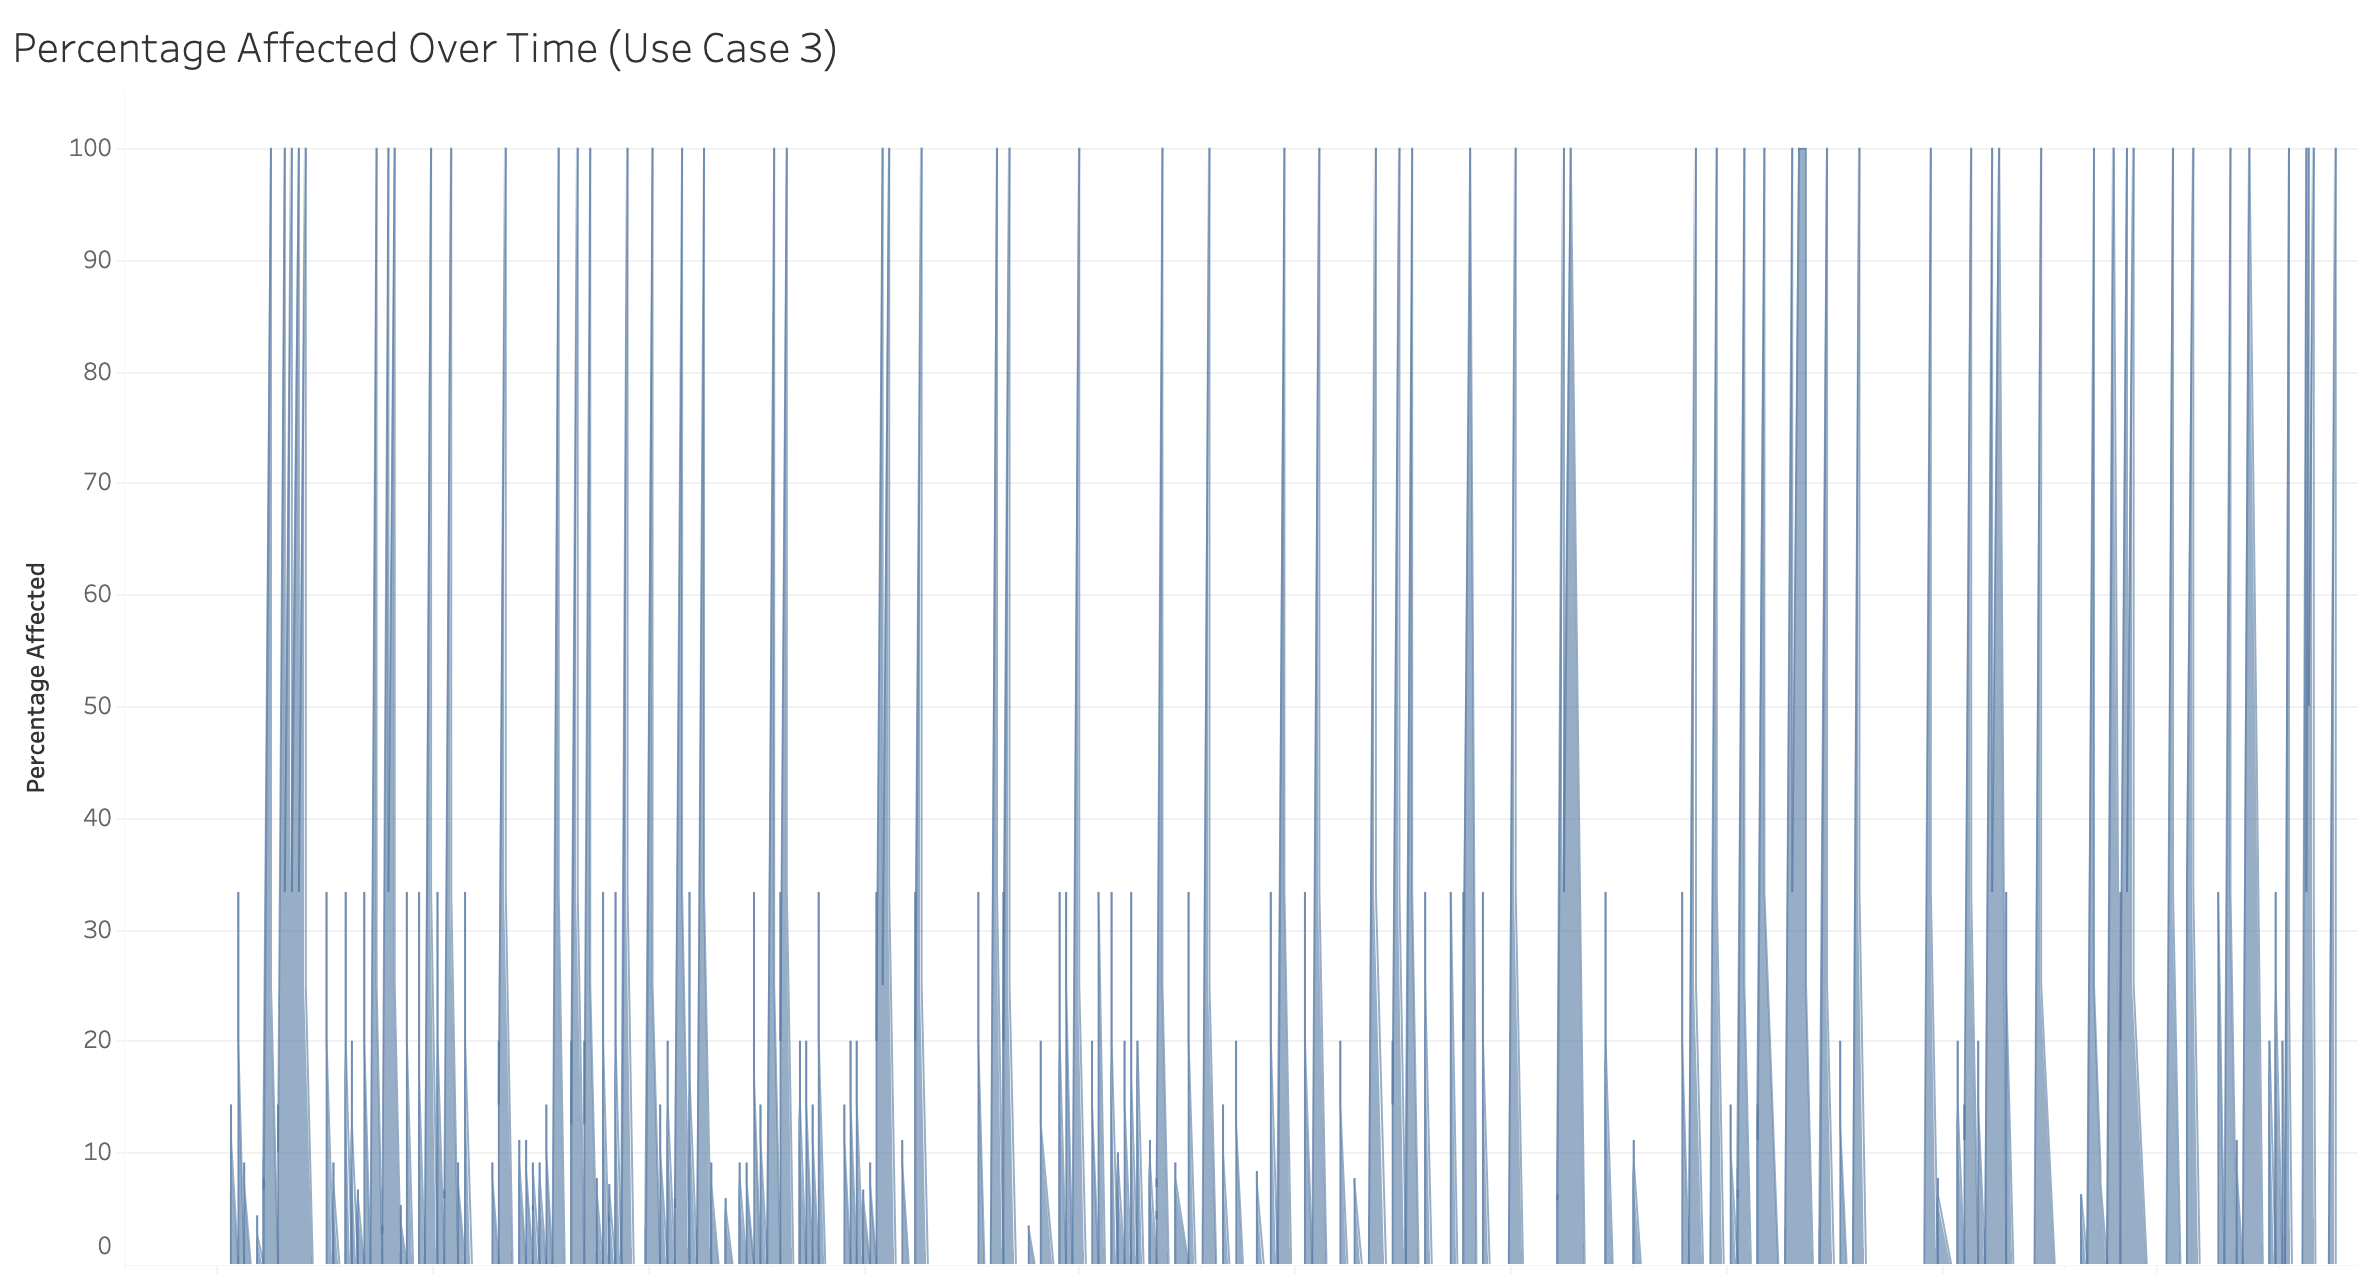
\includegraphics[scale=0.35]{images/UseCase3.png}
\caption{Use Case Gamma}
\label{image:use_case_gamma}
\end{figure}

The final use case of our initial executions was Use Case Delta (shown in Figure \ref{image:use_case_delta}). This use case is very similar to the previous use case and the results show that as well. In this use case we increase the recalculation percentage to 7\% while also increasing the conflicting and abort percentages to 50\%. There is nothing significant to note here other than the findings met our expectations given the parameters.

\begin{figure}
\centering
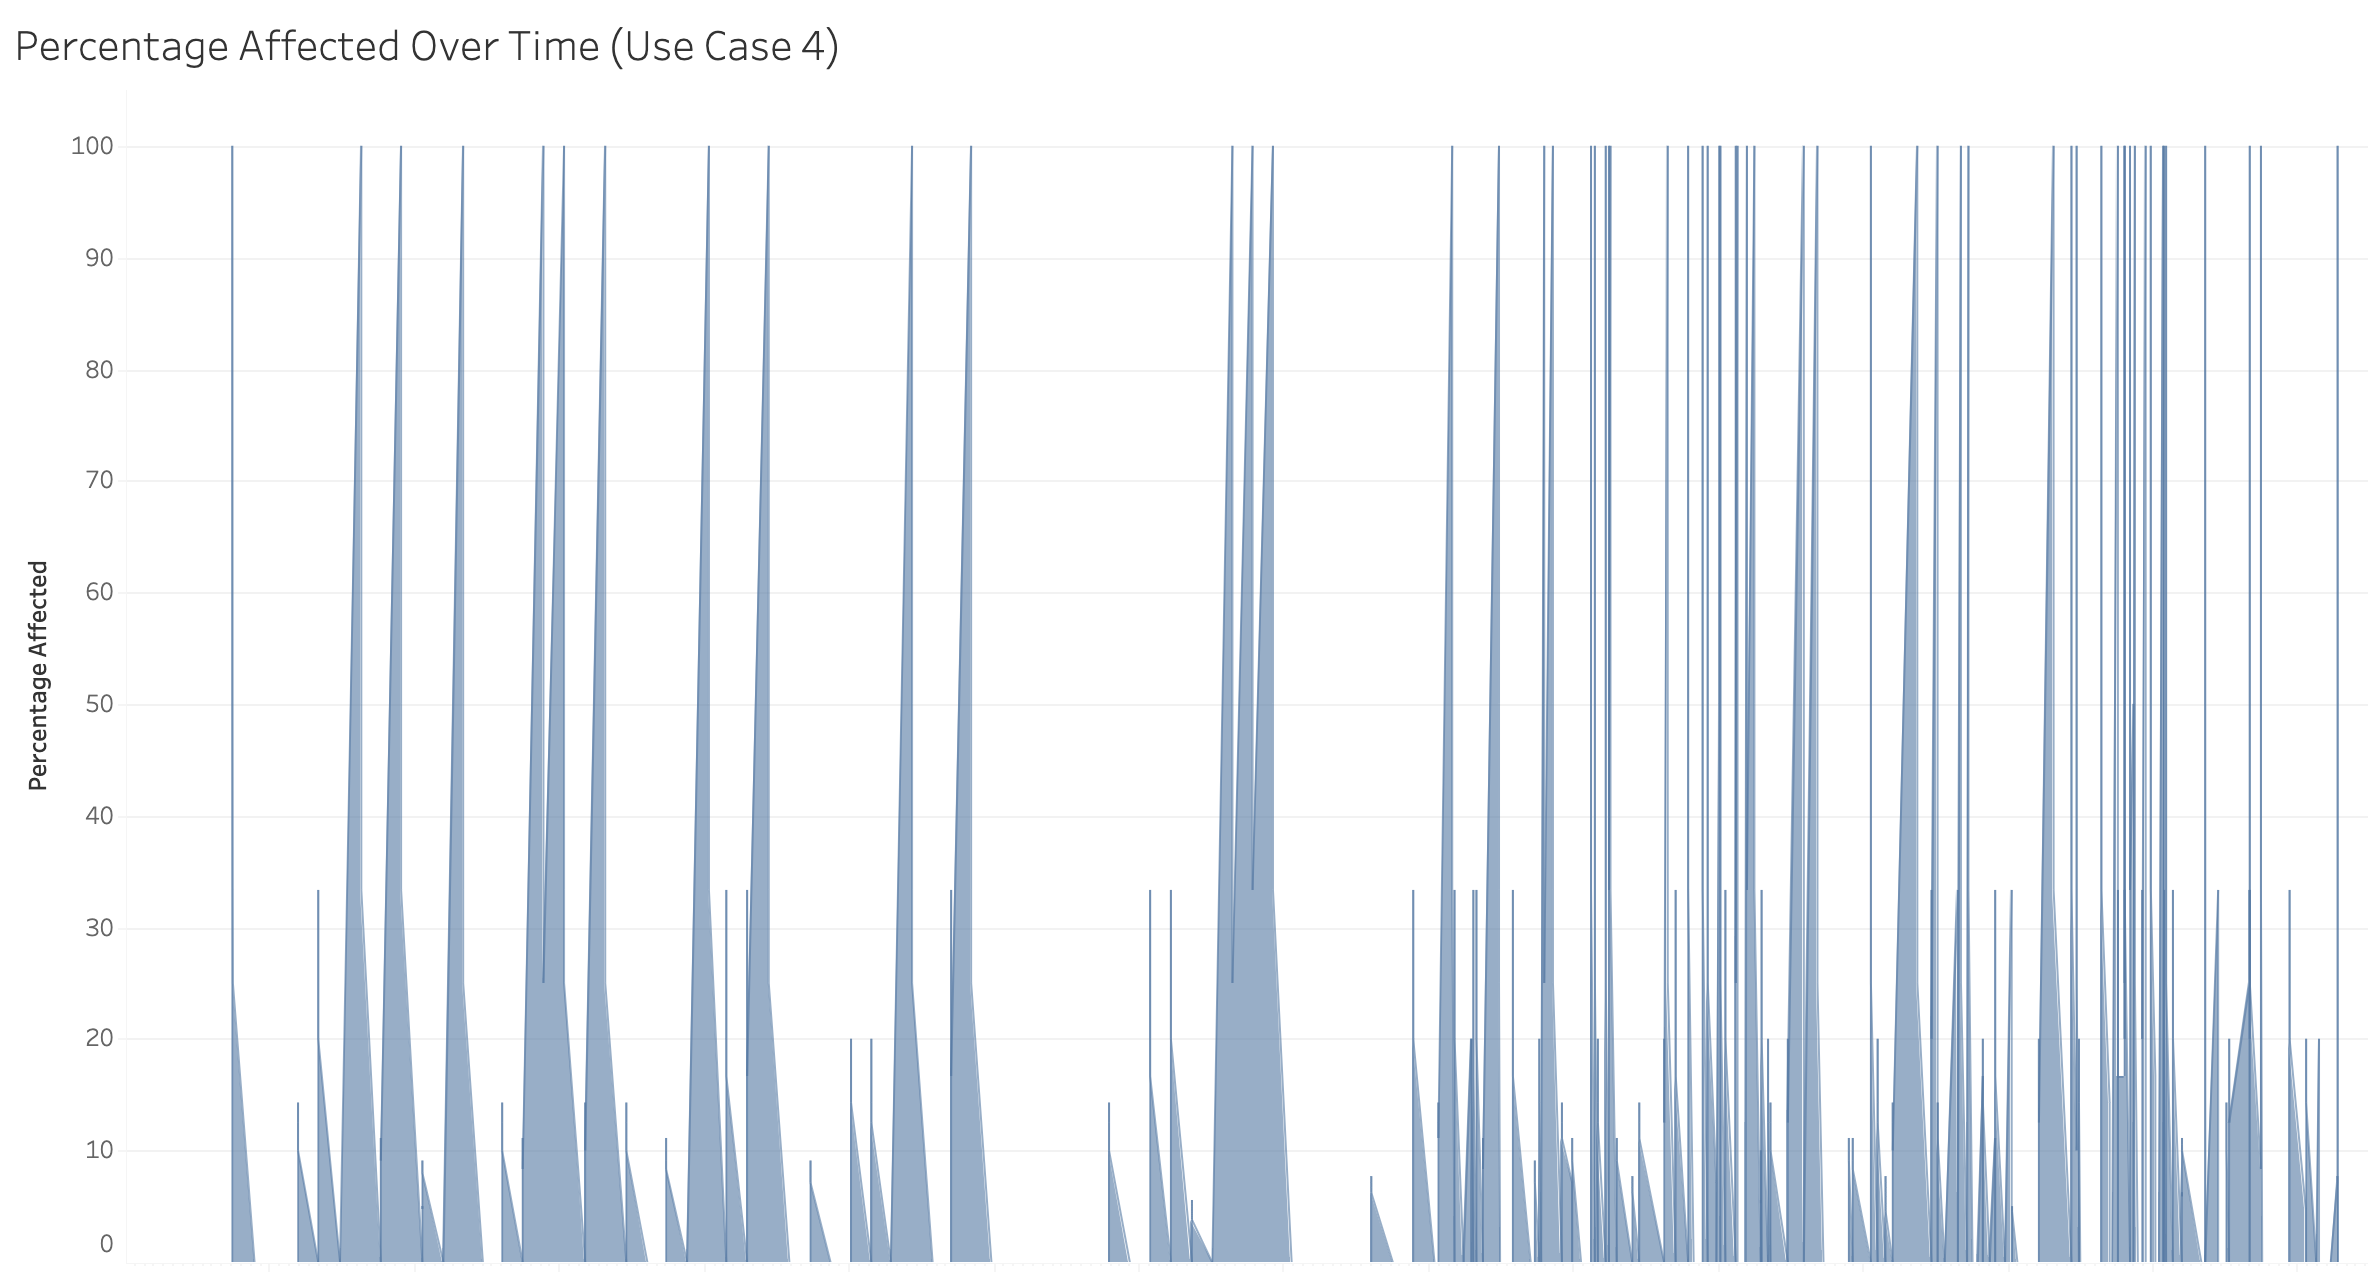
\includegraphics[scale=0.35]{images/UseCase4.png}
\caption{Use Case Delta}
\label{image:use_case_delta}
\end{figure}

After seeing the results of the initial use cases we formulated the use cases documented in Table \ref{tbl:use_cases} to better verify our expectations in Section \ref{sec:anal_expectations}. The next section discusses the actual use cases we used to gather our empirical results.